\subsection{The geometric significance of the dot product}

Given two vectors, $\vect{u}$ and $\vect{v}$, the \textbf{included angle}\index{included angle}
  is the angle between these two vectors which
is given by $\theta$ such that $0 \leq \theta \leq \pi$. The dot product can be used to
determine the included angle between two vectors. Consider the following picture where $\theta$ gives the included angle. 

\begin{center}
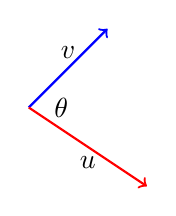
\begin{tikzpicture}
\draw[->, thick, blue](0,0)--(1,1);
\draw[->, thick, red](0,0)--(1.5, -1);
\node[above] at (0.5,0.5){$\vect{v}$};
\node[below] at (0.75, -0.5){$\vect{u}$};
\node[right] at (0.2,0){$\theta$};
\end{tikzpicture}
\end{center}

\begin{proposition}{The dot product and the included angle}{dotproductangle}
Let $\vect{u}$ and $\vect{v}$ be two vectors in $\R^n$, and let 
$\theta$ be the included angle. Then the following equation holds.
\begin{equation*}
\vect{u}\dotprod \vect{v}=\norm{\vect{u}} \norm{\vect{v}
} \cos \theta 
\end{equation*}
\end{proposition}

In words, the dot product of two vectors equals the product of
the magnitude (or length) of the two vectors multiplied by the cosine of the included
angle. Note this gives a geometric description of the dot product which does
not depend explicitly on the coordinates of the vectors.

Consider the following example.

\begin{example}{Find the angle between two vectors}{angletwovectors}
Find the angle between the vectors given by 
\begin{equation*}
\vect{u}
=
\begin{mymatrix}{r}
2 \\
2
\end{mymatrix}, 
\vect{v}
=
\begin{mymatrix}{r}
0 \\
3 
\end{mymatrix}
\end{equation*}
\end{example}

\begin{solution}
By Proposition \ref{prop:dotproductangle},
\begin{equation*}
\vect{u}\dotprod \vect{v}=\norm{\vect{u}} \norm{\vect{v}
} \cos \theta 
\end{equation*}
Hence, 
\begin{equation*}
\cos \theta =\frac{\vect{u}\dotprod \vect{v}}{\norm{\vect{u}} \norm{\vect{v}
}}
\end{equation*}
 
First, we can compute $\vect{u}\dotprod \vect{v}$. By Definition \ref{def:dotproductdefn}, this equals
\begin{equation*}
\vect{u}\dotprod \vect{v}
=
(2)(0) + (2)(3) = 6
\end{equation*}

Then, 
\begin{equation*}
\begin{array}{c}
\norm{\vect{u}}
=
\sqrt{(2)(2)+(2)(2)}=2\sqrt{2}\\
\norm{\vect{v}}
=
\sqrt{(0)(0)+(3)(3)}=\sqrt{3}
\end{array}
\end{equation*}
 Therefore, the cosine of the included angle equals
\begin{equation*}
\cos \theta =\frac{6}{(2\sqrt{2})(3)}=\frac{1}{2}
\end{equation*}

With the cosine known, the angle can be determined by computing the
inverse cosine of that angle, giving approximately  $\theta =\frac{\pi}{4}$ radians. 
\end{solution}

Another application of the geometric description of the dot product is
in finding the angle between two lines. Typically one would assume that the
lines intersect. In some situations, however, it may make sense to ask this
question when the lines do not intersect, such as the angle between
two object trajectories. In any case we understand it to mean the
smallest angle between (any of) their direction vectors. The only
subtlety here is that if $\vect{u}$ is a direction vector for a line,
then so is any multiple $k\vect{u}$, and thus we will find complementary angles
among all angles between direction vectors for two lines, and we
simply take the smaller of the two.

\begin{example}{Find the angle between two lines}{anglebetweentwolines}
Find the angle between the two lines
\begin{equation*}
L_1:  \;
\begin{mymatrix}{r}
x \\
y \\
z 
\end{mymatrix}
 = 
\begin{mymatrix}{r}
1 \\
2 \\
0
\end{mymatrix} +t\begin{mymatrix}{r}
-1 \\
1 \\
2
\end{mymatrix} 
\end{equation*}
 and
\begin{equation*}
L_2: \;
\begin{mymatrix}{r}
x \\
y \\
z
\end{mymatrix}
 = 
\begin{mymatrix}{r}
0 \\
4 \\
-3
\end{mymatrix}
 +s\begin{mymatrix}{r}
2 \\
1 \\
-1
\end{mymatrix}
\end{equation*}
\end{example}

\begin{solution}
You can verify that these lines do not intersect, but as discussed
above this does not matter and we simply find the smallest angle
between any directions vectors for these lines.

To do so  we first find the angle
between the direction vectors given above:
\begin{equation*}
\vect{u}=\begin{mymatrix}{r}
-1 \\
1 \\
2
\end{mymatrix},\;
\vect{v}=\begin{mymatrix}{r}
2 \\
1 \\
-1
\end{mymatrix}
\end{equation*}

In order to find the angle, we solve the following equation for $\theta$
\begin{equation*}
\vect{u}\dotprod \vect{v}=\norm{\vect{u}} \norm{\vect{v}
} \cos \theta
\end{equation*}
to obtain $\cos \theta = -\frac{1}{2}$ and since we choose included
angles between $0$ and $\pi$ we obtain $\theta = \frac{2 \pi}{3}$.


Now the angles between any two direction vectors for these lines will
either be $\frac{2 \pi}{3}$ or its complement $ \phi = \pi -  \frac{2 \pi}{3}
= \frac{\pi}{3}$. We choose the smaller angle, and therefore conclude that the angle between the two lines is $\frac{\pi}{3}$.
\end{solution}

We can also use Proposition \ref{prop:dotproductangle} to compute the dot product of two vectors.

\begin{example}{Using geometric description to find a dot product}{geometricdotproduct}
Let $\vect{u},\vect{v}$ be vectors with $ \norm{\vect{u}} = 3$ and $\norm{\vect{v}} = 4$. 
Suppose the angle between $\vect{u}$ and $\vect{v}$ is $\pi / 3$. Find $\vect{u}\dotprod \vect{v}$.
\end{example}

\begin{solution}
From the geometric description of the dot product in Proposition \ref{prop:dotproductangle}
\begin{equation*}
\vect{u}\dotprod \vect{v}=(3)(4) \cos \tup{\pi / 3} =3\times
4\times 1/2=6
\end{equation*}
\end{solution}

Two nonzero  vectors are said to be \textbf{perpendicular}\index{vector!perpendicular}, sometimes also called \textbf{orthogonal}\index{vector!orthogonal}, if
the included angle is $\pi /2$ radians ($90^{\circ }).$

Consider the following proposition.

\begin{proposition}{Perpendicular vectors}{perpvectors}
Let $\vect{u}$ and $\vect{v}$ be nonzero vectors in $\R^n$. Then, 
$\vect{u}$ and $\vect{v}$ are \textbf{perpendicular}\index{vector!perpendicular} if and only if
\begin{equation*}
\vect{u}
\dotprod
\vect{v}
=
0
\end{equation*}
\end{proposition}

\begin{proof}
This follows directly from Proposition \ref{prop:dotproductangle}. First if the dot product of
two nonzero vectors is equal to $0$, this tells us that $\cos \theta
=0$ (this is where we need nonzero vectors). Thus $\theta = \pi /2$
and the vectors are perpendicular.

If on the other hand $\vect{v}$ is perpendicular to $\vect{u}$, then 
the included angle is $\pi /2$ radians. Hence $\cos \theta =0$ and 
$\vect{u} \dotprod \vect{v} = 0$.
\end{proof}

Consider the following example.

\begin{example}{Determine if two vectors are perpendicular}{perpendicularvectors}
Determine whether the two vectors, 
\begin{equation*}
\vect{u}=
\begin{mymatrix}{r}
2 \\
1 \\
-1 
\end{mymatrix}, 
\vect{v} 
=
\begin{mymatrix}{r}
1 \\
3 \\
5
\end{mymatrix}
\end{equation*}
 are perpendicular.
\end{example}

\begin{solution}
In order to determine if these two vectors are perpendicular, we compute the dot product.
This is given by
\begin{equation*}
\vect{u} \dotprod \vect{v}
=
(2)(1) + (1)(3) + (-1)(5)
=
0
\end{equation*}
Therefore, by Proposition \ref{prop:perpvectors} these two vectors are perpendicular.
\end{solution}
